\subsection{Bedienung}
Die Software zur Bedienung wurde in drei Teile gestaltet. Hardwaremäßig wurde nur das geringste an Elemente verwendet. Die drei Bedienelemente sind jeweils Aktiv High am Mikrocontroller geschaltet mittels einem Taster-Pull-Up-Schaltkreis \ref{fig:SwitchPullUp_Software}. Der Pull-Up Widerstand ist 10k\Omega, der mit einem Taster auf Erde geschaltet wird.

\begin{figure}[h]
	\centering
		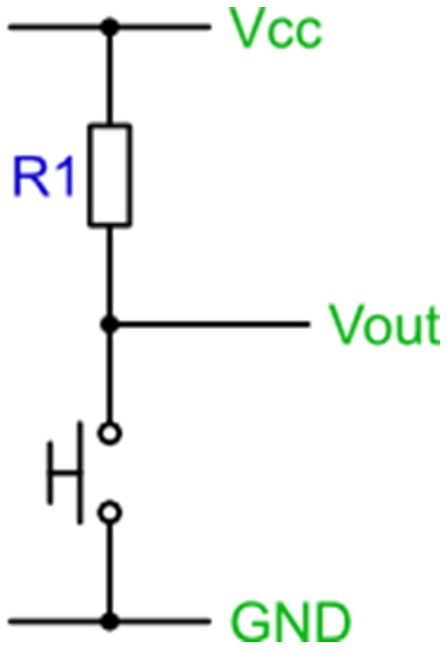
\includegraphics[width=1.00\textwidth]{switchpullupcircuit.jpg}
	\caption{Taster-Pull-Up-Schaltkreis}
	\label{fig:SwitchPullUp_Software}
\end{figure}

Der Mikrocontroller fragt den Taster Eingang mit einem Timer-Interrupt alle 16ms ab und übergibt das Signal einer Funktion zur Entprellung der Taster. Die Funktion durchläuft eine for-Schleife, die das Signal nach Einsen (1) und Nullen sortiert. Überwiegen nach N-Wiederholungen die Einsen ist der Taster gedrückt und die hinterlegte Aktion wird aktiviert. \newline
%Die Taster können zweifach verwendet werden. Einerseits kann der Taster kurzzeitig ged%